\documentclass[a4paper,11pt]{article}
\usepackage[margin=2.5cm]{geometry}
\usepackage[authoryear,round]{natbib}
\usepackage{graphicx}
\usepackage{booktabs}
\usepackage{array}
\usepackage{tabularx}
\usepackage{longtable}
\usepackage{xspace}
\usepackage{xcolor}
\usepackage[colorlinks=true,allcolors={blue!60!black}]{hyperref}
%% Dibuat otomatis oleh tools/scopus/angka_naskah.py; jangan disunting manual.
%% Setiap makro adalah satu angka korpus yang dihitung dari literature/scopus-2026-09.
\newcommand{\kHumElig}{0.45\xspace}
\newcommand{\kHumTitles}{0.57\xspace}
\newcommand{\nAbsIncl}{1{,}013\xspace}
\newcommand{\nApp}{64\xspace}
\newcommand{\nAppOnly}{0\xspace}
\newcommand{\nAppTrack}{57\xspace}
\newcommand{\nAppWith}{64\xspace}
\newcommand{\nAssessed}{1{,}145\xspace}
\newcommand{\nAwaiting}{0\xspace}
\newcommand{\nClassAfter}{3\xspace}
\newcommand{\nClassDuring}{10\xspace}
\newcommand{\nClassPerDet}{1\xspace}
\newcommand{\nClassSingle}{33\xspace}
\newcommand{\nClassSingleBlueberry}{5\xspace}
\newcommand{\nClassSingleMaturity}{28\xspace}
\newcommand{\nClassSingleTomato}{10\xspace}
\newcommand{\nClassUnstated}{14\xspace}
\newcommand{\nClassVote}{5\xspace}
\newcommand{\nCodedAbs}{0\xspace}
\newcommand{\nCodedFull}{240\xspace}
\newcommand{\nCodedTitle}{0\xspace}
\newcommand{\nCombined}{95\xspace}
\newcommand{\nCropApple}{71\xspace}
\newcommand{\nCropCitrus}{28\xspace}
\newcommand{\nCropGrape}{24\xspace}
\newcommand{\nCropMango}{15\xspace}
\newcommand{\nCropStrawberry}{13\xspace}
\newcommand{\nCropTomato}{31\xspace}
\newcommand{\nDepth}{94\xspace}
\newcommand{\nDepthApple}{33\xspace}
\newcommand{\nDepthLidar}{6\xspace}
\newcommand{\nDepthRgbd}{62\xspace}
\newcommand{\nDepthStereo}{13\xspace}
\newcommand{\nDiscrete}{30\xspace}
\newcommand{\nDiscreteGeom}{15\xspace}
\newcommand{\nDiscreteStat}{15\xspace}
\newcommand{\nDocType}{166\xspace}
\newcommand{\nEarly}{15\xspace}
\newcommand{\nEarlyGeom}{11\xspace}
\newcommand{\nEarlyStat}{4\xspace}
\newcommand{\nEarlyTrack}{2\xspace}
\newcommand{\nEligExcl}{132\xspace}
\newcommand{\nExclEight}{0\xspace}
\newcommand{\nExclFive}{60\xspace}
\newcommand{\nExclFour}{1\xspace}
\newcommand{\nExclOne}{23\xspace}
\newcommand{\nExclSeven}{1\xspace}
\newcommand{\nExclSix}{4\xspace}
\newcommand{\nExclThree}{25\xspace}
\newcommand{\nExclTwo}{18\xspace}
\newcommand{\nFTAssessed}{845\xspace}
\newcommand{\nFTExcl}{26\xspace}
\newcommand{\nFTExclEight}{2\xspace}
\newcommand{\nFTExclFive}{12\xspace}
\newcommand{\nFTExclFour}{0\xspace}
\newcommand{\nFTExclOne}{1\xspace}
\newcommand{\nFTExclSeven}{0\xspace}
\newcommand{\nFTExclSix}{0\xspace}
\newcommand{\nFTExclThree}{2\xspace}
\newcommand{\nFTExclTwo}{9\xspace}
\newcommand{\nFullText}{819\xspace}
\newcommand{\nGeom}{99\xspace}
\newcommand{\nGeomOnly}{66\xspace}
\newcommand{\nHumElig}{165\xspace}
\newcommand{\nHumEligAgree}{86\xspace}
\newcommand{\nHumTitles}{300\xspace}
\newcommand{\nHumTitlesAgree}{256\xspace}
\newcommand{\nIdentTermMax}{33\xspace}
\newcommand{\nIdentTermMin}{24\xspace}
\newcommand{\nIncluded}{819\xspace}
\newcommand{\nKelasBanding}{7\xspace}
\newcommand{\nKelasLain}{15\xspace}
\newcommand{\nKelasLainTengah}{9\xspace}
\newcommand{\nKelasLebih}{6\xspace}
\newcommand{\nKelasTengah}{11\xspace}
\newcommand{\nKelasTiga}{21\xspace}
\newcommand{\nKelasUnik}{6\xspace}
\newcommand{\nKelasUnikMentah}{3\xspace}
\newcommand{\nKelasUnikTengah}{2\xspace}
\newcommand{\nLearn}{8\xspace}
\newcommand{\nLearnOnly}{0\xspace}
\newcommand{\nLinks}{289\xspace}
\newcommand{\nMetCount}{197\xspace}
\newcommand{\nMetCountOnly}{52\xspace}
\newcommand{\nMetDet}{163\xspace}
\newcommand{\nMetIdent}{77\xspace}
\newcommand{\nMetNone}{6\xspace}
\newcommand{\nMethod}{235\xspace}
\newcommand{\nMethodMetric}{235\xspace}
\newcommand{\nModLidar}{10\xspace}
\newcommand{\nModMulti}{5\xspace}
\newcommand{\nModRgb}{190\xspace}
\newcommand{\nModRgbd}{18\xspace}
\newcommand{\nModStereo}{8\xspace}
\newcommand{\nMulti}{240\xspace}
\newcommand{\nMultiData}{5\xspace}
\newcommand{\nMultiEarlyMax}{9\xspace}
\newcommand{\nMultiFullText}{240\xspace}
\newcommand{\nMultiNoFullText}{0\xspace}
\newcommand{\nMultiPeak}{55\xspace}
\newcommand{\nMultiScopus}{239\xspace}
\newcommand{\nNoAbstract}{254\xspace}
\newcommand{\nNone}{1\xspace}
\newcommand{\nNoneOnly}{1\xspace}
\newcommand{\nNotRetrieved}{173\xspace}
\newcommand{\nNotRetrievedClass}{12\xspace}
\newcommand{\nNotRetrievedDepth}{30\xspace}
\newcommand{\nNotRetrievedMulti}{1\xspace}
\newcommand{\nNotRetrievedPalm}{48\xspace}
\newcommand{\nNotRetrievedReview}{17\xspace}
\newcommand{\nNotRetrievedSingle}{60\xspace}
\newcommand{\nNotRetrievedTransfer}{5\xspace}
\newcommand{\nOther}{5\xspace}
\newcommand{\nOtherComb}{16\xspace}
\newcommand{\nOtherRetrieved}{5\xspace}
\newcommand{\nOutside}{83\xspace}
\newcommand{\nPalm}{122\xspace}
\newcommand{\nPalmCls}{57\xspace}
\newcommand{\nPalmCount}{3\xspace}
\newcommand{\nPalmData}{4\xspace}
\newcommand{\nPalmDet}{22\xspace}
\newcommand{\nPalmField}{19\xspace}
\newcommand{\nPalmGround}{9\xspace}
\newcommand{\nPalmInstClass}{97\xspace}
\newcommand{\nPalmLoose}{4\xspace}
\newcommand{\nPalmMill}{40\xspace}
\newcommand{\nPalmMixed}{5\xspace}
\newcommand{\nPalmOnTree}{17\xspace}
\newcommand{\nPalmQual}{16\xspace}
\newcommand{\nPalmSensor}{16\xspace}
\newcommand{\nPalmUav}{2\xspace}
\newcommand{\nPalmUnstated}{22\xspace}
\newcommand{\nPalmViews}{17\xspace}
\newcommand{\nPalmWeb}{8\xspace}
\newcommand{\nPerClass}{33\xspace}
\newcommand{\nPlatGround}{91\xspace}
\newcommand{\nPlatHand}{52\xspace}
\newcommand{\nPlatLab}{1\xspace}
\newcommand{\nPlatNone}{38\xspace}
\newcommand{\nPlatSeveral}{16\xspace}
\newcommand{\nPlatUav}{32\xspace}
\newcommand{\nRecent}{155\xspace}
\newcommand{\nRefAnnot}{143\xspace}
\newcommand{\nRefHarvest}{43\xspace}
\newcommand{\nRefNone}{23\xspace}
\newcommand{\nRefPack}{2\xspace}
\newcommand{\nRefTree}{56\xspace}
\newcommand{\nRetrieved}{6{,}491\xspace}
\newcommand{\nReviews}{105\xspace}
\newcommand{\nRevisit}{5\xspace}
\newcommand{\nSampleTitles}{300\xspace}
\newcommand{\nSampleTitlesEligible}{11\xspace}
\newcommand{\nScan}{41\xspace}
\newcommand{\nScopusIncl}{814\xspace}
\newcommand{\nSingle}{142\xspace}
\newcommand{\nSingleView}{0\xspace}
\newcommand{\nSought}{1{,}018\xspace}
\newcommand{\nStat}{22\xspace}
\newcommand{\nStatOnly}{19\xspace}
\newcommand{\nTermCounting}{363\xspace}
\newcommand{\nTermDetection}{495\xspace}
\newcommand{\nTerms}{42\xspace}
\newcommand{\nTitleExcl}{4{,}578\xspace}
\newcommand{\nTitleRecheck}{1{,}325\xspace}
\newcommand{\nTitleReinstated}{19\xspace}
\newcommand{\nTitles}{5{,}723\xspace}
\newcommand{\nTrack}{141\xspace}
\newcommand{\nTrackGeom}{22\xspace}
\newcommand{\nTrackGeomScan}{7\xspace}
\newcommand{\nTrackGeomVideo}{15\xspace}
\newcommand{\nTrackOnly}{54\xspace}
\newcommand{\nUnique}{5{,}889\xspace}
\newcommand{\nVideo}{159\xspace}
\newcommand{\nWithAbstract}{665\xspace}
\newcommand{\nYearFirst}{8\xspace}
\newcommand{\nYearPeak}{140\xspace}
\newcommand{\pApp}{27}
\newcommand{\pAppRecent}{33}
\newcommand{\pGeom}{42}
\newcommand{\pHumElig}{52}
\newcommand{\pHumTitles}{85}
\newcommand{\pLearn}{3}
\newcommand{\pMetCount}{84}
\newcommand{\pMetDet}{69}
\newcommand{\pMetIdent}{33}
\newcommand{\pMetNone}{3}
\newcommand{\pNone}{0}
\newcommand{\pNotRetrieved}{17}
\newcommand{\pStat}{9}
\newcommand{\pTrack}{60}
\newcommand{\pTrackRecent}{70}

\graphicspath{{../figures/main6/}}
\newcolumntype{Y}{>{\raggedright\arraybackslash}X}
\newcolumntype{L}[1]{>{\raggedright\arraybackslash}p{#1}}
\renewcommand{\thesection}{S\arabic{section}}
\renewcommand{\thefigure}{S\arabic{figure}}
\renewcommand{\thetable}{S\arabic{table}}
\renewcommand{\figurename}{Fig.}
\title{Supplementary Material\\[4pt]\large Cross-view identity in image-based fruit counting: A systematic review and a design space for class-wise inventories}
\author{Muhammad Zainal Muttaqin and Fatma Indriani}
\date{}
\begin{document}
\maketitle

This supplement gives the procedural details of the review that the main article summarizes in its Review method section, and the descriptive figures that support the quantitative profile. Section numbers of the main article are referred to by name.

\section{Screening procedure}\label{sup:screening}

\textit{Deduplication and document types.} Duplicates were removed by Scopus record identifier. Proceedings front matter, errata, notes, editorials, letters, and retracted items were removed by document type before title screening. For the three largest query sets (oil-palm imaging, depth and 3D sensing, and reviews of fruit detection and yield), titles were sorted by keyword so that similar titles were read together.

\textit{Abstracts.} The Scopus export used did not contain abstracts. Abstracts were compiled from OpenAlex, Semantic Scholar, Crossref, and Europe PMC. For \nNoAbstract records no abstract could be found; these were assessed from the title, the source, and, where available, the summary provided by Semantic Scholar.

\textit{Model-assisted screening and second pass.} A large language model read each title and abstract and recorded a decision and a group. All multi-observation and oil-palm studies and all exclusions at the eligibility stage were checked in a second pass without access to the first decisions, and disagreements were resolved against the source.

\textit{Re-check of title exclusions.} Because title screening missed some eligible records, the abstracts of all \nTitleRecheck title-stage exclusions from the multi-observation and oil-palm query sets were read, and \nTitleReinstated records were included. In a random sample of \nSampleTitles title exclusions from all query sets, \nSampleTitlesEligible met an inclusion criterion once their abstracts were read; title exclusions from the remaining query sets were not re-read.

\textit{Human check.} The first author screened random samples of \nHumTitles titles and \nHumElig eligibility records without seeing the model's decisions. Agreement was \pHumTitles\% for titles (Cohen's $\kappa$ = \kHumTitles) and \pHumElig\% for eligibility codes ($\kappa$ = \kHumElig).

\textit{Reports from outside the search.} Outside the search, \nOther reports were identified: one review of citrus yield prediction published online before the search date but assigned to a 2027 volume, and four studies found by checking the reference lists of the five closest reviews for multi-observation studies that the search had missed. Of these, \nOtherRetrieved were retrieved, assessed in full text, and entered the map.

\textit{Full-text assessment.} The \nFTAssessed retrieved reports were read in full by the language model, which reported for each one the group, any reason for exclusion, and the passages that supported them. Every proposed exclusion or change of group was checked against those passages in the full text in a second pass. The reviewer approved the resulting decisions.

\section{Coding rules}\label{sup:coding}

\textit{Group precedence.} Where a study met the definition of more than one group, the multi-observation group took precedence for any study that combines several observations of the same fruit. A stereo image pair was treated as a single observation: a study that detects, locates, or sizes fruit from one stereo pair was assigned to the depth and 3D sensing group, and to the multi-observation group only when it links fruit across frames or across camera positions.

\textit{Association mechanism.} A study that uses several mechanisms was assigned each of them, so mechanism totals are occurrences, not exclusive study counts. Linking between consecutive frames by motion or overlap was coded as temporal tracking. Trackers that add an appearance descriptor to the motion model, such as DeepSORT and StrongSORT, were coded as appearance matching combined with temporal tracking. Tracking followed by 3D localization was coded as temporal tracking combined with geometric association. A fitted factor applied after individual fruit were linked was recorded with the linking mechanism, not as statistical correction \citep{nuske2014modeling,wang2013automated}. Identity taken from physical tags on the fruit was coded as no association, because no observation was linked from the images \citep{kassim2012oil}. A study that fuses images from several positions into a 3D model, panorama, or orthomosaic and detects or counts fruit in that model was coded as geometric association. A study that combines counts or features from two or more images of the same plant by a fitted or learned rule, without linking individual fruit, was coded as statistical correction; plain summation was coded as no association. A calibration applied to counts that another mechanism has already made unique was not coded as statistical correction, because it does not decide identity.

\textit{Scope of the multi-observation group.} A study that tracks fruit across frames was included as a multi-observation study only when the tracking or a count was evaluated. Dataset papers without an association method were coded separately and are not included in the mechanism statistics.

\textit{Acquisition and classes.} Acquisition was coded as a 3D scan when fruit were detected or counted in a point cloud or 3D model, and as revisits over time only when the identity of a fruit was linked across visits. Counts per class were coded only when a study reports counts, not only detections, for each class.

\textit{Supporting groups.} The single-view counting, single-image class-wise counting, depth and 3D sensing, review, and outside-agriculture groups were coded by keyword rules for crop, modality, platform, and class attribute, and the rule output was spot-checked; the group of each of these studies was confirmed on its full text at the eligibility stage.

\textit{Unit of counting.} The unit is the report. A report that reprints another included report, such as a book chapter that repeats a journal article, is linked to it and counted once (main text, Section~2.3). Reports that share a pipeline or data but are not reprints of one another are counted separately. Examples are a conference paper and a journal article by the same authors on the same apple-counting pipeline \citep{osman2021yieldb,osman2021yield}, and three reports on the same apple orchard datasets that give the same fruit counts after the two sides of a row are merged \citep{roy2019vision,dong2020semantic,hani2020comparative}.

\begin{table}[ht]
\centering
\caption{Questions of the review, the groups of included studies that answer them, and the sections of the main article where they are answered.}\label{tab:rqmap}
\footnotesize
\begin{tabularx}{\textwidth}{@{}L{4.6cm}L{3.6cm}YL{2.6cm}@{}}
\toprule
Question or purpose & Main evidence & Supporting groups & Sections\\
\midrule
(1) Mechanisms and the conditions each assumes & Multi-observation studies & Depth and 3D sensing studies; methods papers from outside agriculture & Design space; Association; Depth\\
(2) How well each mechanism works, and how that was measured & Multi-observation studies & Single-view counting studies, as a baseline & Acquisition; Association\\
(3) Classes on unique fruit & Multi-observation studies that report counts per class & Single-image class-wise counting studies & Class attributes\\
(4) The oil-palm case & Oil-palm studies & None & Oil palm\\
Positioning & Earlier reviews & None & Discussion\\
\bottomrule
\end{tabularx}
\end{table}

\section{Term co-occurrence map}\label{sup:terms}

A term co-occurrence map was computed from the titles and available abstracts of the \nIncluded included studies (\nWithAbstract have an abstract; the others contribute their title only). A fixed vocabulary of task, method, sensor, and crop terms was matched in each record. Terms found in at least 20 studies were kept, two terms were linked when at least 12 studies contained both, and terms were grouped by modularity clustering on association strength. The map was used for orientation only and did not affect inclusion.

Fig.~\ref{fig:terms} shows \nTerms terms and \nLinks links. Its three large clusters match the groups of the review: counting, yield estimation, video, and tracking sit together with the terms for identity (data association, double counting, multi-view) and with 3D reconstruction; depth, red-green-blue-depth (RGB-D) imaging, stereo, and point clouds sit with apple, orchard, occlusion, and localization; and ripeness, classification, and grading sit with oil palm. A fourth, small cluster joins tomato and greenhouse. Each identity term occurs in \nIdentTermMin to \nIdentTermMax of the \nIncluded studies, against \nTermDetection for detection and \nTermCounting for counting.

\begin{figure}[ht]
\centering
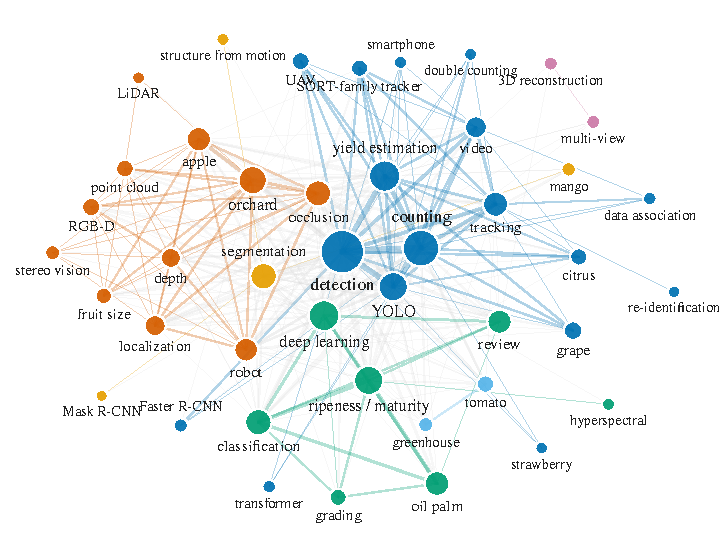
\includegraphics[width=0.9\textwidth]{F08_istilah}
\caption{Term co-occurrence map of the included studies, where node size, line width, and colour represent the number of studies containing the term in the title or abstract, the number of studies containing both terms, and the cluster, respectively.}\label{fig:terms}
\end{figure}

\section{Crops, platforms, and sensors of the method studies}\label{sup:landscape}

Fig.~\ref{fig:crop} relates crop to association mechanism. Apple accounts for \nCropApple of the \nMethod method studies, citrus for \nCropCitrus, grape for \nCropGrape, tomato for \nCropTomato, strawberry for \nCropStrawberry, and mango for \nCropMango.

Fig.~\ref{fig:sensor} gives modality and platform by crop. Crop and platform were read from the full text of each study: the crop whose fruit the study itself detected, counted, or tracked, and what carried the camera when its images were taken. Of the \nMethod method studies, \nPlatNone do not state the platform, \nPlatGround used a ground vehicle or robot, \nPlatUav an unmanned aerial vehicle (UAV), \nPlatHand a handheld device or smartphone, and \nPlatSeveral more than one platform; each study is counted once. Modality was coded by keyword rules from titles and abstracts: a red-green-blue (RGB) camera is the sensor in \nModRgb studies; RGB-D cameras appear in \nModRgbd, stereo cameras in \nModStereo, light detection and ranging (LiDAR) in \nModLidar, and multispectral cameras in \nModMulti. The modality counts describe what abstracts report, not what was used.

\begin{figure}[ht]
\centering
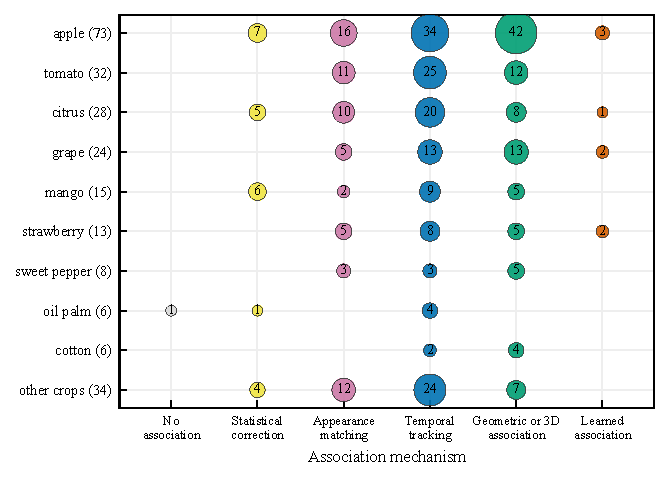
\includegraphics[width=0.7\textwidth]{F05_tanaman_mekanisme}
\caption{Multi-observation method studies by crop and association mechanism ($n=\nMethod$), where the number in each circle is the study count.}\label{fig:crop}
\end{figure}

\begin{figure}[ht]
\centering
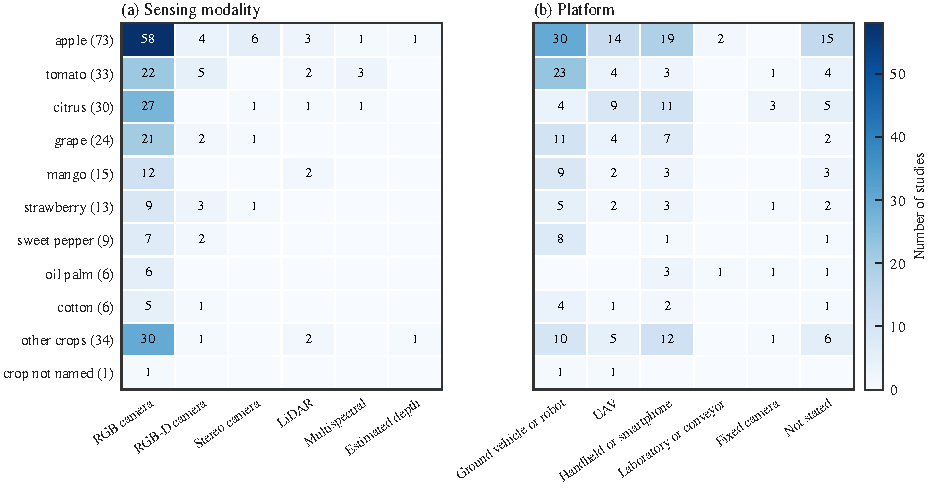
\includegraphics[width=\textwidth]{F10_sensor}
\caption{Sensing modality and platform by crop in the multi-observation method studies ($n=\nMethod$): (a) modality; (b) platform.}\label{fig:sensor}
\end{figure}

\section{PRISMA 2020 checklist}\label{sup:prisma}

Table~\ref{tab:prisma} gives the location of each item of the PRISMA 2020 checklist \citep{page2021prisma} in the main article or in this supplement. Item texts are abbreviated. Items about pooled results are marked as not applicable because the review is a mapping review that does not pool effect sizes.

\begin{footnotesize}
\setlength{\tabcolsep}{3pt}
\begin{longtable}{@{}L{3.0cm}L{0.8cm}L{6.4cm}L{5.6cm}@{}}
\caption{PRISMA 2020 checklist with the location where each item is reported.}\label{tab:prisma}\\
\toprule
Section and topic & Item & Checklist item & Location\\
\midrule
\endfirsthead
\toprule
Section and topic & Item & Checklist item & Location\\
\midrule
\endhead
\bottomrule
\endfoot
Title & 1 & Identify the report as a systematic review. & Title\\
Abstract & 2 & Report the abstract according to the PRISMA 2020 for Abstracts checklist. & Abstract\\
Introduction: rationale & 3 & Describe the rationale for the review in the context of existing knowledge. & Section 1; Section 9.3\\
Introduction: objectives & 4 & State the objectives or questions the review addresses. & Section 1, questions (1)--(4)\\
Methods: eligibility criteria & 5 & Specify the inclusion and exclusion criteria and how studies were grouped for the syntheses. & Section 2.2; Section 2.4 and Table 2\\
Methods: information sources & 6 & Specify all sources searched or consulted and the date each was last searched. & Section 2.1 (Scopus, 28 September 2026); Section 2.3 and Section S1 (reference lists of the closest reviews)\\
Methods: search strategy & 7 & Present the full search strategies, including filters and limits. & Table 1; Appendix B\\
Methods: selection process & 8 & Specify how inclusion was decided: number of reviewers, independence, and automation tools. & Section 2.3; Section S1\\
Methods: data collection process & 9 & Specify how data were collected: number of reviewers, independence, and automation tools. & Section 2.4; Section S2; declaration of generative AI\\
Methods: data items & 10a & List and define the outcomes for which data were sought. & Section 2.4, items (iv)--(vi); Section 2.5 (metrics)\\
 & 10b & List and define the other variables for which data were sought. & Section 2.4, items (i)--(iii); Sections S2 and S4\\
Methods: risk of bias in studies & 11 & Specify the methods used to assess risk of bias in the included studies. & Section 2.5: no quality score per study; for each comparison the count reference, whether arms used the same data, the metric level, and whether the favoured arm was the authors' own were recorded and enter the certainty grade\\
Methods: effect measures & 12 & Specify the effect measures used for each outcome. & Section 2.5: metrics as reported by each study; no pooled effect measure\\
Methods: synthesis methods & 13a & Describe how studies were selected for each synthesis. & Section 2.4 (groups); Section 2.5 (conditions for a comparison on the same data)\\
 & 13b & Describe any preparation of data for presentation or synthesis. & Section 2.5 (fractions converted to percentages)\\
 & 13c & Describe how results were tabulated or displayed. & Section 2.5; Tables 3--5; Figs.~4--7\\
 & 13d & Describe the synthesis methods and their rationale. & Section 2 (configurative synthesis without pooling); Section 2.5 (structured narrative)\\
 & 13e & Describe methods used to explore heterogeneity among results. & Section 2.5; Table 5, last column\\
 & 13f & Describe any sensitivity analyses. & Not applicable: no results were pooled\\
Methods: reporting bias assessment & 14 & Describe methods used to assess the risk of bias due to missing results. & Not assessed; retrieval bias is discussed in Section 10\\
Methods: certainty assessment & 15 & Describe methods used to assess certainty in the body of evidence. & Section 2.5: each main finding graded high, moderate, or low by a fixed rule on supporting and opposing research groups, crops, field references, and whether a method other than the authors' own was favoured\\
Results: study selection & 16a & Describe the results of the search and selection, ideally with a flow diagram. & Section 2.3; Fig.~1\\
 & 16b & Cite studies that might appear to meet the criteria but were excluded, and explain why. & Supplementary Data S1 (reports excluded at full text, with reasons); Section 2.3 (second reports of included studies)\\
Results: study characteristics & 17 & Cite each included study and present its characteristics. & Supplementary Data S1; Appendix Table A1; Section 3.4; Section S4\\
Results: risk of bias in studies & 18 & Present assessments of risk of bias for each included study. & Tables 3 and 5 (count reference, same data, metric level); Section 5.6\\
Results: individual studies & 19 & Present the results of each study for each outcome. & Tables 3 and 5; Appendix Table A1\\
Results: syntheses & 20a & Summarize the characteristics and risk of bias of the studies in each synthesis. & Sections 3.4 and 5.6\\
 & 20b & Present the results of all statistical syntheses. & Not applicable: no results were pooled\\
 & 20c & Present the results of investigations of heterogeneity. & Sections 4 and 5; Table 5\\
 & 20d & Present the results of sensitivity analyses. & Not applicable: no results were pooled\\
Results: reporting biases & 21 & Present assessments of risk of bias due to missing results. & Not assessed; Section 10\\
Results: certainty of evidence & 22 & Present assessments of certainty in the body of evidence. & Table 6 and Section 9.2\\
Discussion & 23a & Provide a general interpretation of the results. & Section 9\\
 & 23b & Discuss limitations of the evidence included in the review. & Sections 5.6 and 9.4\\
 & 23c & Discuss limitations of the review processes used. & Section 10\\
 & 23d & Discuss implications for practice, policy, and future research. & Sections 9.4, 9.5, and 11\\
Other information: registration and protocol & 24a & Provide registration information or state that the review was not registered. & Section 2: not registered\\
 & 24b & Indicate where the protocol can be accessed or state that none was prepared. & Section 2: no protocol was registered or published; screening and coding rules are given in Sections S1 and S2\\
 & 24c & Describe and explain any amendments to the registration or protocol. & Not applicable; changes to codes made during verification are recorded in the change log (Section S6)\\
Other information: support & 25 & Describe sources of financial or non-financial support. & Funding\\
Other information: competing interests & 26 & Declare any competing interests of the review authors. & Declaration of competing interest\\
Other information: availability of data, code, and materials & 27 & Report which data, code, and materials are publicly available and where. & Data availability; Section S6\\
\end{longtable}
\end{footnotesize}

\section{Files provided}\label{sup:files}

Supplementary Data S1 is a table in comma-separated values format with one row for each of the \nFTAssessed reports assessed in full text: the \nIncluded included studies, ordered by group, followed by the \nFTExcl reports excluded at the full-text stage. Its columns give the status (included or excluded at full text), the group, the reason for exclusion in the words of the flow diagram, the first author, year, title, source, and digital object identifier, the association mechanism and acquisition design of each multi-observation study, and whether the study is cited in the main article.

The screening decision for every record, the coded evidence matrix, the log of changes made during verification, and the analysis scripts that reproduce the numbers and figures of the main article are provided with this supplement.

\bibliographystyle{cas-model2-names}
\bibliography{references6}
\end{document}
